% (C) Marc Lijour, 2016-2017 
% Licensed under a Creative Commons License BY-SA
% https://creativecommons.org/licenses/by-sa/2.5/ca/
% Presentation for the Small Business Digitization Initiative (SBDI) training program
% see http://www.ictc-ctic.ca/small-business-digitization-initiative/ 
% authored by Marc Lijour, December 2016
% for the session running from January 2017 to September 2017
% 
% ======================================================================================================
%                                   PROGRAM OVERVIEW
% ======================================================================================================
\section{Program Overview}
% --------------------- Purpose of the Program --------------------------
\subsection{Purpose of the Program}
\begin{frame}[c]{Small Business Digitization Initiative}
	\centering
	\Huge{Welcome!}
\end{frame}

\frame{
	\frametitle{Small Business Digitization Initiative}
	\framesubtitle{A Sense of Purpose}
	\begin{figure}
	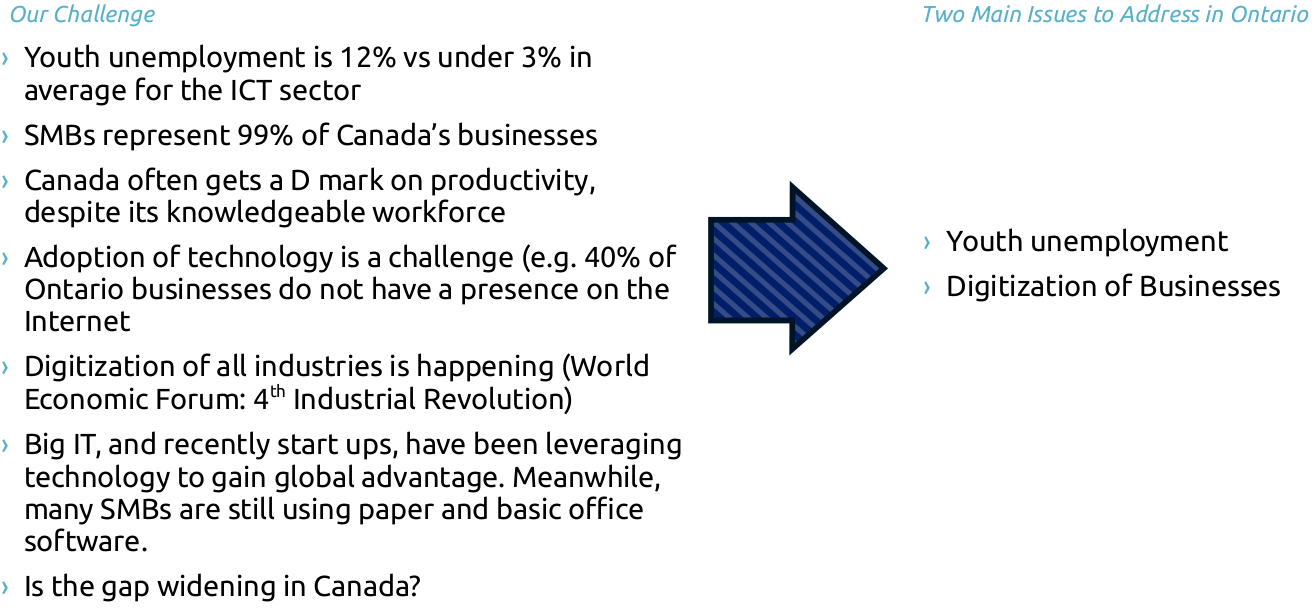
\includegraphics[width=12cm]{../pics/SBDI-purpose}
	\end{figure}
}

\frame{
	\frametitle{Small Business Digitization Initiative}
	\framesubtitle{A Case Study - part 1: Typical SMB Challenge}
	\begin{itemize}
		\item Wholesale Fruits and Vegetable company, about 25 employees
		\pause
		\item Family-run business, which grew organically over time
		\pause
		\item Staff did not have any idea at which price to buy and sell to make their margin
		\pause
		\item Executives did not know if they were losing or making money on specific lines of product
	\end{itemize}
}

\frame{
	\frametitle{Small Business Digitization Initiative}
	\framesubtitle{A Case Study - part 2: Solution}
%	\begin{block}{Solution}
	Savoir-faire Linux digitized key business processes to improve productivity:
%	\end{block}
	\begin{itemize}
		\item \emph{Analytical Accounting} to allow executives to make more informed decisions
		\pause
		\item \emph{Real-time Pricing} data made available through mobile apps to buyers and seller
		\pause
		\item \emph{Location Tracking} of the shipping crates in the refrigerated trucks, to facilitate partial recalls when necessary
		\pause
		\item More \emph{Back-Office Automation} to save staff time (labelling, invoicing, etc)
	\end{itemize}
}

\frame{
	\frametitle{Small Business Digitization Initiative}
	\framesubtitle{A Case Study - part 3: Results}
	\begin{block}{Results}
	The Company saved 20\% of their FTE time (about 5 employees).\\
	Moving these employees to Sales generated a \$15 million/year increase in revenues.
	\end{block}
}

\frame{
	\frametitle{Small Business Digitization Initiative}
	\framesubtitle{Governments and Industry alike are Responding}
	\begin{figure}
	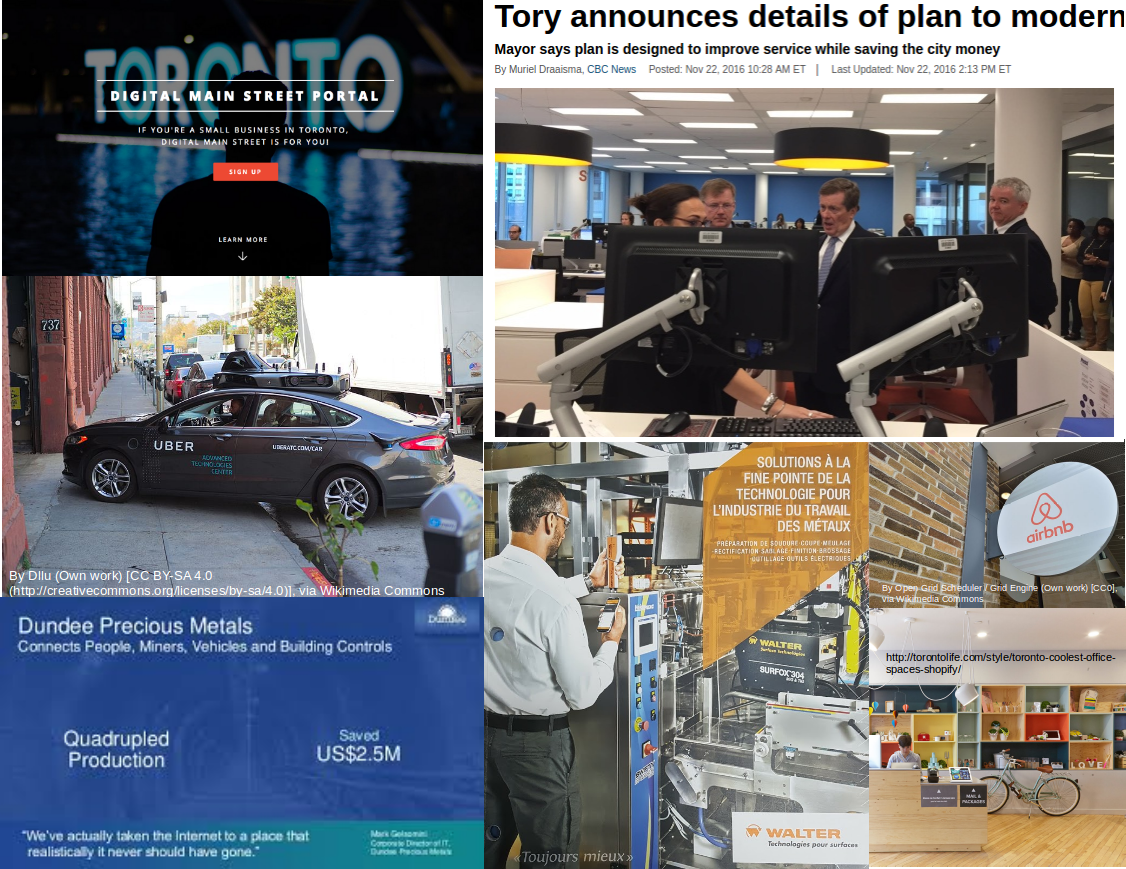
\includegraphics[width=10cm]{../pics/patchwork-digitization-in-Toronto}
	\end{figure}
}

\frame{
	\frametitle{Small Business Digitization Initiative}
	\framesubtitle{Challenges \& Opportunities}
	\begin{itemize}
		\item The pace of change is accelerating (e.g. Technology time to market)
		\pause 
		\item Technology enables disruptive innovation
		\pause
		\item Businesses don't understand fully the potential \& benefits
		\pause
		\item There are not enough workers capable of designing \& implementing digitized solutions
		\pause
		\item Change is hard. IT Change is especially risky \& difficult (Software Crisis).
		\pause
		\item SMBs can't rely on the same resources as a Google, Facebook, Twitter...
		\pause
		\item other?
	\end{itemize}
}

\frame{
	\frametitle{Small Business Digitization Initiative}
	\framesubtitle{Opportunities for Ontario (and Ontarians)}
	Can we lead the Digital Revolution?
	\begin{columns}
	\column{0.5\textwidth}
		\begin{figure}
		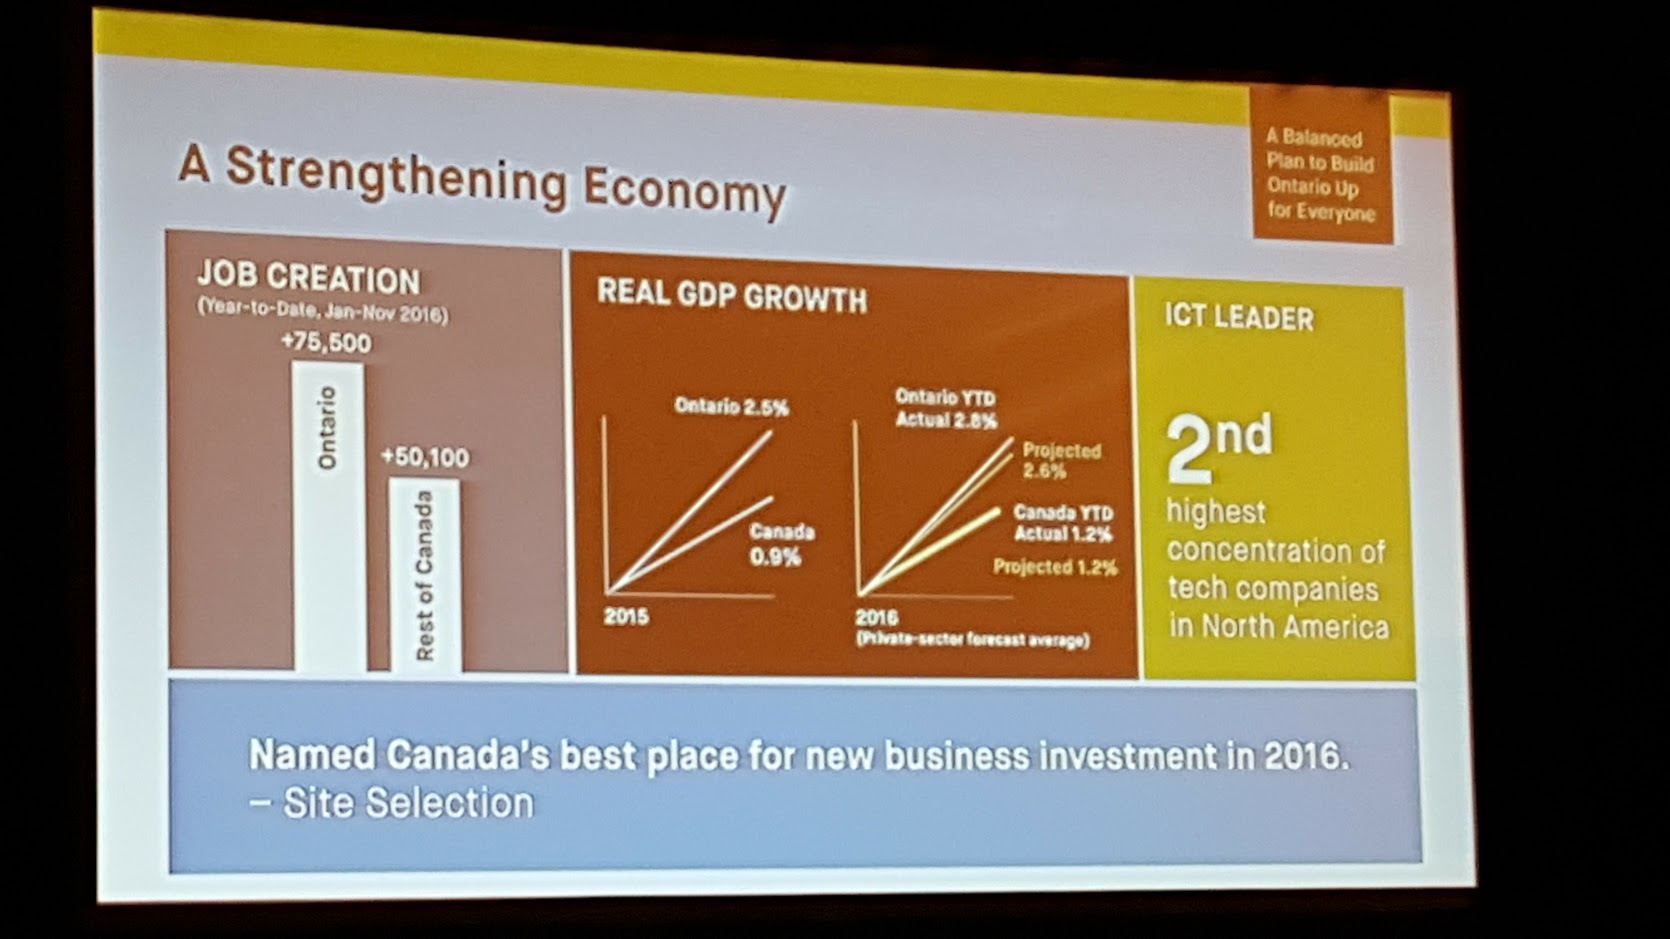
\includegraphics[width=7cm]{../pics/Wynne-economy-2016}
		\end{figure}
	\column{0.5\textwidth}
		\begin{figure}
		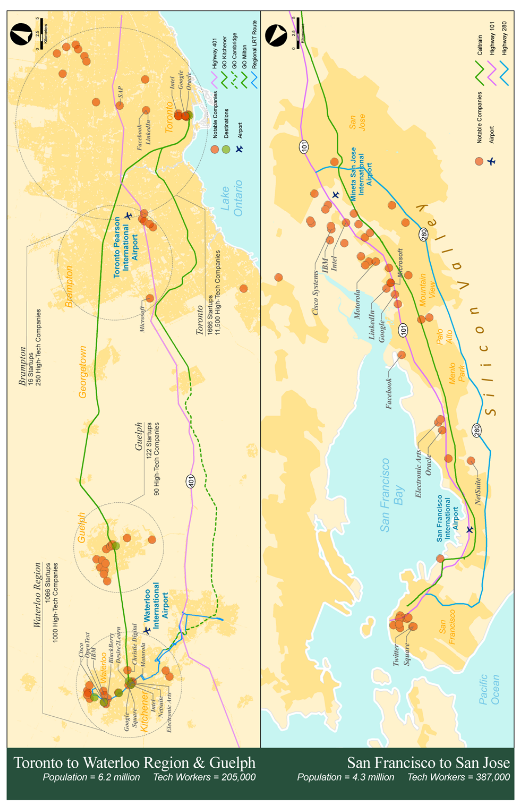
\includegraphics[width=3cm]{../pics/Toronto-Waterloo-corridor}
		\end{figure}
	\end{columns}
}
% --------------------- Description of the course --------------------------
\subsection{Organization of the Program \& Expectations}
\begin{frame}[c]{Small Business Digitization Initiative}
	\centering
	\Huge{Course Organization \& Expectations}\\
	\vspace{3em}
	{\tiny Note. The SBDI Training program is property of ICTC. All rights reserved.}
\end{frame}

\frame{
	\frametitle{Small Business Digitization Initiative}
	\framesubtitle{Main Components of the Course}
	\begin{figure}
	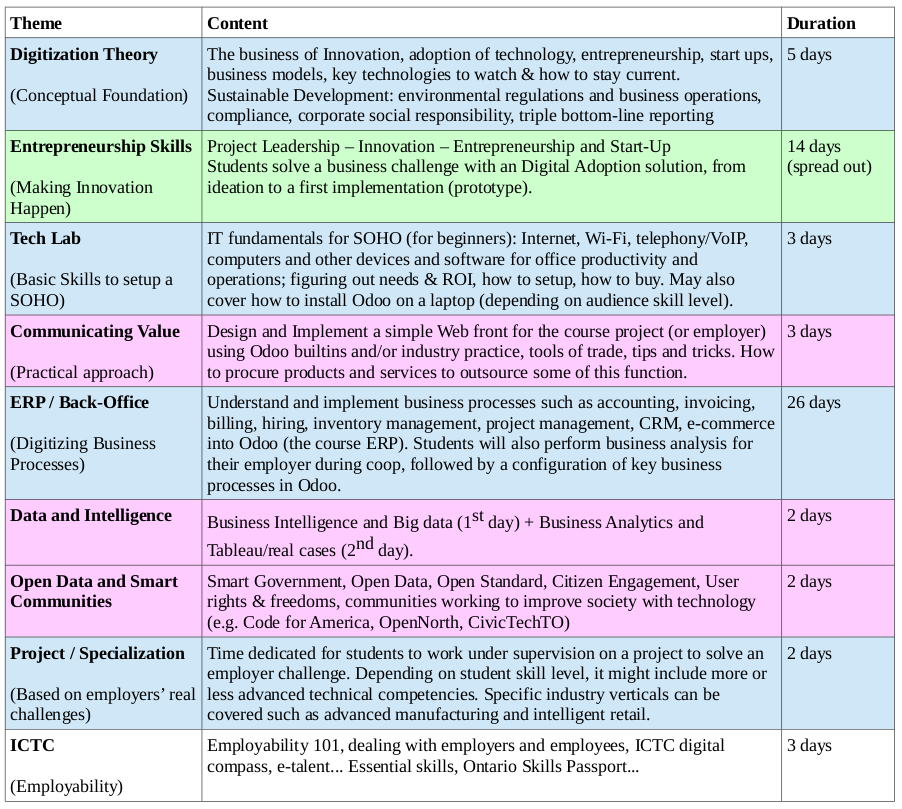
\includegraphics[height=7.5cm]{../pics/SBDI-overview-table}
	\end{figure}
}

\frame{
	\frametitle{Small Business Digitization Initiative}
	\framesubtitle{Odoo -- The course ``ERP''}
	\begin{figure}
	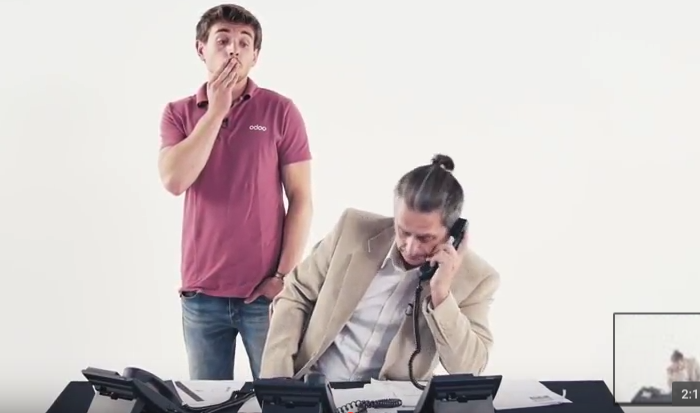
\includegraphics[width=11.5cm]{../pics/odoo-youtube-notERP}
	\caption{\tiny\url{https://www.youtube.com/watch?v=2dhyhamLm6M&list=PL1-aSABtP6AALA_4hW2TyYIioOVEGQ3yf&index=6}}
	\end{figure}
}

\frame{
	\frametitle{Small Business Digitization Initiative}
	\framesubtitle{Course Sequence}
	\begin{figure}
	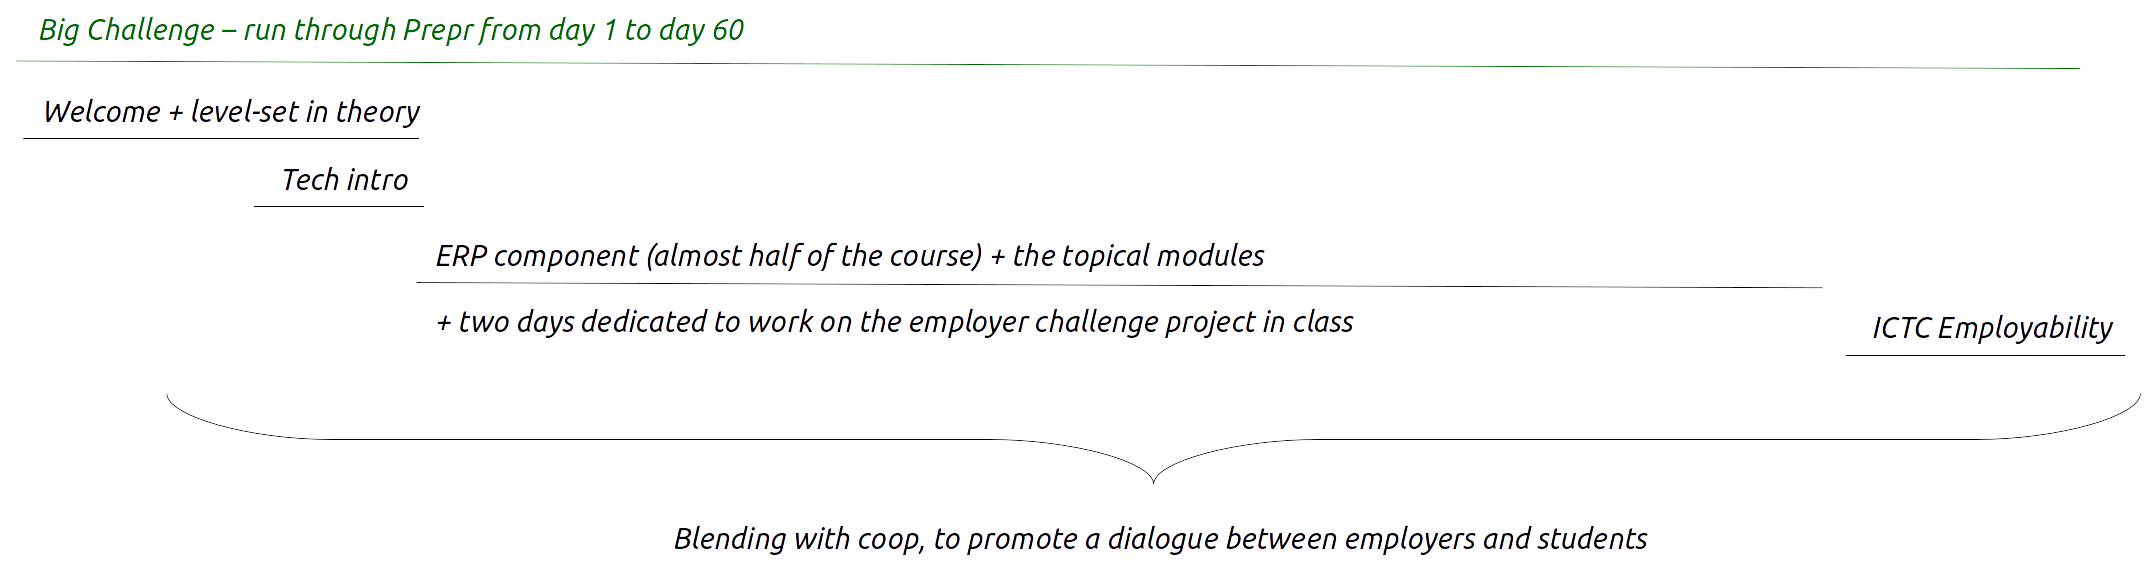
\includegraphics[width=12cm]{../pics/SBDI-course-linear-view}
	\end{figure}
}

\frame{
	\frametitle{Small Business Digitization Initiative}
	\framesubtitle{Class Time}
	\begin{table}
	\begin{tabular}{l | c}
	Time & Activity \\
	\hline \hline
	9am - 10:30am 		& Class\\
	10:30am			& Break\\
	10:40am - 12:10pm	& Class\\
	12:10pm			& Lunch\\
	12:50pm - 2:20pm	& Class\\
	2:20pm			& Break\\
	2:30pm - 4pm		& Class\\
	\end{tabular}
	\end{table}
}

\frame{
	\frametitle{Small Business Digitization Initiative}
	\framesubtitle{Work placement}
	\begin{block}{Employer Challenge}
	Opportunity to leverage \emph{i)} the theory learned in class and \emph{ii)} the intimate understanding of your employer's job functions and business processes, to design new ways to improve their business by leveraging digital technology.
	\end{block}
	\begin{alertblock}{Job Skills}
	During the work placement, you are expected to behave as a regular employee or consultant. That means \emph{i)} a high standard of professionalism, and \emph{ii)} the performance of work duties that are valuable to the business. You will deliver a report, and if possible a working prototype, to your ``customer'' at the end of the course.
	\end{alertblock}
}

\frame{
	\frametitle{Small Business Digitization Initiative}
	\framesubtitle{ERP Component (26 days)}
	\begin{itemize}
		\item Opportunity to study how a business works (complementing the work placement)
		\pause
		\item Focusing on eight business functions:
		\begin{enumerate}
			\item Introduction to ERP + Customer Relationship Management (CRM)
			\item Sales Management
			\item Purchasing Management
			\item Manufacturing Management
			\item Inventory Management
			\item Accounting Management
			\item Project Management
			\item Human Resources Management
		\end{enumerate}
		\pause
		\item The study of each module will be broken down in 3 steps:
		\begin{description}
			\item[Day 1:] Theory, key concepts, best practices
			\item[Day 2:] Introduction to Odoo (the course ERP)
			\item[Day 3:] Analyzing business processes
		\end{description}
		\item See next slides
	\end{itemize}
}

\frame{
	\frametitle{Small Business Digitization Initiative}
	\framesubtitle{Business Module - Day 1 (key concepts)}
	\begin{itemize}
		\item Primer on (8) main business functions
		\pause
		\item Best practices in the industry
		\pause
		\item Reflection about process variation (e.g. FIFO vs. LIFO)
	\end{itemize}
}

\frame{
	\frametitle{Small Business Digitization Initiative}
	\framesubtitle{Business Module - Day 2 (the tools of the trade)}
	\begin{itemize}
		\item Introduction to Odoo -the ERP system used for this course
		\pause
		\item \href{https://www.odoo.com}{Odoo} is a fresh and flexible ERP under an \href{https://github.com/odoo/odoo/blob/10.0/LICENSE}{Open Source license}% (LGPLv3)}
		\pause
		\item The \href{https://odoo-community.org}{Odoo Community Association} is a good place for support and community-supported apps
		\pause
		\item Your instructors support the community in a number of ways, e.g. with the \href{https://www.meetup.com/Odoo-Toronto/}{Odoo Toronto Meetup}
		\pause
		\item You will have 8 days of training on Odoo (one per each module) 
		\pause
		\item Across these 8 days, you'll follow the journey of a fictitious company implementing an ERP
		\pause
		\item You will have access to 2 databases (one for class, one for the work placement)
		\pause
		\item Start becoming familiar with Odoo today!\\(\href{https://www.youtube.com/user/OpenERPonline}{Youtube} is a good place to start)
	\end{itemize}
}

\frame{
	\frametitle{Small Business Digitization Initiative}
	\framesubtitle{Business Module - Day 3 (initiating the digitization journey)}
	\begin{itemize}
		\item This is where theory meets skills and good understanding of the business at your work placement
		\pause
		\item You'll work in a workshop format to conceptualize the business processes observed at the work place (your ``customer'')
		\pause
		\item Producing diagrams and other documents describing the \emph{as-is} and \emph{to-be} state of the process
		\pause
		\item Discussing potential improvements (based on industry best practices, capabilities of Odoo, etc)
		\pause
		\item Working towards implementing some of these processes in Odoo and
		\item Preparing a report for the business (your ``customer'')
	\end{itemize}
}

\frame{
	\frametitle{Small Business Digitization Initiative}
	\framesubtitle{Special Project (2 days)}
	\begin{itemize}
		\item Extra days to help you complete the Employer Challenge
		\pause
		\item Can be used to 
			\begin{itemize}
				\item refine the business analysis
				\item implement some processes in Odoo
				\item complete the report for your ``customer''
			\end{itemize}
		\pause
	\end{itemize}
	\begin{alertblock}{Attention}
		Don't underestimate the importance of a thorough business analysis. The main cause of IT project failures is a lack of solid and sound requirements.\\
		Remember: \centering\\Project done right $\neq$ the Right Project is done!
	\end{alertblock}
}

\frame{
	\frametitle{Small Business Digitization Initiative}
	\framesubtitle{Business Analysis 101 (2 days)}
	\begin{itemize}
		\item Solid foundations 
		\pause
		\item Before you start the work placement
		\pause
		\item Techniques to explore your ``customer'' business processes in a thorough \& professional way
		\pause
		\item Techniques to conceptualize and to represent a process on paper
		\pause
		\item The documentation you produce will be foundational both to your report and to working on a prototype
	\end{itemize}
}

\frame{
	\frametitle{Small Business Digitization Initiative}
	\framesubtitle{Other Modules}
	\begin{itemize}
		\item To build awareness on business areas that will be impacted by your work
			\begin{itemize}
				\item Communications, Sales \& Marketing\\
					(e.g. can you enable a new line of revenue?)
				\item Big Data \& Analytics\\
					(e.g. can you surface intelligence to allow more informed decisions?)
				\item Open Data \& Smart Communities\\
					(e.g. can you leverage Open Data for your ``customer''?)
			\end{itemize}
	\end{itemize}
}

\begin{frame}[c]{Small Business Digitization Initiative}
	\centering
	\Huge{Are you ready?}
\end{frame}

\frame{
	\frametitle{Small Business Digitization Initiative}
	\framesubtitle{Let's Start!}
	\begin{itemize}
		\item Download these slides at \url{http://bit.ly/sbditheoryday1}
		\item Form teams of 4
		\item Fill the form at \url{https://goo.gl/forms/moKSrsmIepUaqjFX2} (contact info, background \& interests, team)
		\item Discuss in teams: \emph{What is the biggest challenges for SMBs today?}
		\item Pick a spokeperson to share with the class
	\end{itemize}
}

%\frame{
%	\frametitle{}
%	\framesubtitle{}
%}

